\Large{\textbf{Análisis de la complejidad computacional del algoritmo Minimax en el algoritmo \emph{juego m,n,k}}}

\normalsize
\section{Introducción}
El juego es parte fundamental de las sociedades y las culturas del hombre.
Naturalmente existen de diversos tipos, pero lo que todos tienen en común es el
hecho de que estimulan el pensamiento estratégico de  los jugadores. Por lo
tanto, la investigación sobre cómo maximizar la probabilidad de victoria en
ellos ha sido objeto de estudio por siglos. No en balde la rama de probabilidad
inició como una descripción de los juegos de azar. 

Por esta misma razón, desde el surguimiento de las computadoras, uno de los
principales objetivos de los computólogos ha sido la creación de inteligencias
artificiales programadas para resolver este tipo de problemas. Por esta razón
comenzó a interesarme el tema del algoritmo \emph{Minimax}, ya que me parece un
procedimiento cuyo planteamiento es simultáneamente simple y poderoso. El área
de inteligencia artificial, que combina de manera interdisciplinaria
concocimientos de distintas ramas, como matemáticas e informática, me parece
sumamente interesante, y siempre ha llamado mi atención. Recuerdo la fascinación
que produjo en mí aprender sobre el enfrentamiento entre la computadora Deep
Blue y el maestro Garry Kasparov, durante el cuál se desafió el escepticismo de
muchos ante las posibilidades que podrían brindar las computadoras analizando
situaciones complejas como el juego de ajedrez. 

Sin embargo los juegos no son más que una planta de desarrollo, ya que los
principios detrás de los algoritmos utilizados, por ejemplo, la rama
matemática detrás de la estrategia que muchos utilizan, teoría de juegos, fue responsable por algunas
decisiones importantes durante la guerra fría, y resulta una herramienta
efectiva para la toma de decisiones bajo diversas circunstancias. 

De esta manera, decidí indagar sobre las técnicas fundamentales detrás del éxito
revolucionario de Deep Blue, esta investigación me llevó a aprender, entre otras
cosas, sobre la
estrategia \emph{Minimax} y sobre la teoría detrás de esta misma. Y debido a  mi profundo interés en
la programación me percaté de que implementar un algoritmo similar seria un
excelente reto para aprender más sobre los fundamentos de una de las ramas que
me parecen más interesantes del desarrollo tecnológico contemporáneo. 

Lo que me propuse en esta investigación fue aprender sobre el algoritmo \emph{Minimax}
e implementarlo en un pequeño programa, ya que de esta manera podría obtener un conocimiento más personal del mismo al expresarlo en mi propio código. Asímismo, me interesó conocer
sobre su comportamiento bajo distintos escenarios, particularmente sobre los
requerimientos computacionales de tiempo y espacio para hallar la solución
óptima bajo distintos escenarios y determinar las posibles limitaciones del procedimiento. En otras palabras, comprobar experimentalmente lo que en ciencias de la computación se conoce como la  \emph{complejidad asintótica} del algoritmo. 

\clearpage
\section{Sobre los juegos}
Para lograr este objetivo, decidí comenzar investigando los juegos de \emph{Gato} y  \emph{Conecta-4}, ya que . Ambos pertenecen a la familia de los juegos de conección y similares en naturaleza. Esto es porque pueden ser generalizados como un único juego abstracto, conocido como \emph{juego m,n,k}, donde \emph{m} y \emph{n} son el número de columnas y filas en el tablero, y \emph{k} sería el número de fichas que los jugadores deben conectar. Así, el juego de \emph{Gato} sería el juego \emph{3,3,3}, el juego de Conecta-4 \emph{7,6,4} con la adicional regla de limitar hacia el eje horizontal los posibles movimientos del jugador. 

Por la relativa simplicidad del juego de \emph{gato}, decidí utilizarlo únicamente como una base de análisis, y partir de ahí para observar el crecimiento en la complejidad de los juegos y el algoritmo.

Adicionalmente, el juego \emph{juego m,n,k} podría ser caracterizado como un juego \emph{no cooperativo} entre dos jugadores y de \emph{suma cero}, \emph{secuencial} de \emph{información perfecta}. 
En otras palabras, en un juego \emph{juego m,n,k}, existen dos jugadores, max y min, que toman turnos para poner fichas en un tablero, y la utilidad final del juego para cada jugador se cancela entre sí. 

Por ejemplo, en el juego de gato, si un jugador gana, el otro pierde y viceversa; en el caso alternativo, ambos empatan con utilidades iguales. Formalmente, la utilidad  $u$ del jugador $i_{1}$ con respecto a la del jugador $i_{2}$ en un estado $s$ sería la siguiente:

\begin{equation}
u_{i_{1}}(s)=-u_{2_{1}}(s)
\end{equation}

Por lo tanto:

\begin{equation}
u_{i_{1}}(s)+u_{2_{1}}(s) = 0
\end{equation}

Para que un juego deba considerarse de suma cero, esta propiedad debe mantenerse en todos los estados posibles del juego, de tal manera que se cumpla lo siguiente:

\begin{equation}
\forall s \in S, \sum_{a=1}^{n}{u_{i_{1}}(s)}+{u_{i_{2}}(s)}=0
\end{equation}

En otras palabras, en todo juego posible, la utilidad final de un jugador cancela la del otro, o que exactamente lo que uno gana, pierde el otro.

\section{La estrategia minimax}
En consecuencia de lo anterior, la estrategia óptima de cada jugador intenará maximizar su propia ganancia minimizando la de su contrincante, ese es el núcleo de la estrategia minimax. Y su principal utilidad es que por medio de esta, el jugador $i_{x}$ puede garantizar su utilidad mínima de manera independiente de la estrategia de su adversario, en otras palabras, prepararse adecuadamente para el peor escenario (uno en el cuál compita contra otro jugador óptimo).

Para visualizarla, es conveniente utilizar un grafo dirigido representando las posibles decisiones decisiones de los jugadores, formalmente conocido como o arbol de juego, en donde cada arista representa una decisión, y cada vértice un estado de juego. 


Por ejemplo, supongamos que un juego secuencial de información perfecta y  dos jugadores, $\gamma_{1}$, tiene el siguiente arbol dirigido, $G = (V,E)$, cuyo conjunto de vértices $V$, representa los  estados posibles del juego, $S(\gamma_{1})$. Los cuadrados y círulos en los vértices representan respectivamente, momentos en los  que los jugadores $i_{1}$ e $i_{2}$ deben realizar una jugada. 
Estas acciones son representadas en el grafo por el conjunto de aristas $E$. Como el juego se da por turnos, cada decisión contiene el subgrafo resultante $H_{s}(V',E') \in G$, donde $E'$ representa las posibles acciones del jugador y $V'$, el estado del juego después de dicha acción. Y los números, ubicados en nodos terminales --donde acaba el juego--, representan la utilidad $u(s)$ del jugador $i_{1}$\footnote{Como es un juego de suma cero, la utilidad del jugador $i_{2}$ sería sencillamente el inverso aditivo de la utilidad del jugador $i_{2}$, o en la gráfica $-u(s)$}. 

\begin{figure}[h]
\centering
\scalebox{0.95}
{
\begin{forest}
sn edges
[$v_{1}$,rectangle,draw
    [$v_{2}$,circle,draw, edge label={node[midway,left=1.0mm,font=\scriptsize]{$e_{1}$}}
        [$v_{4}$,rectangle,draw, edge label={node[midway,left=1.0mm,font=\scriptsize]{$e_{3}$}}
            [5, 
            %regular polygon,draw, 
            edge label={node[midway,below =1mm,font=\scriptsize]{$e_{9}$}}
            ]
            [1, 
            %regular polygon,draw,
            edge label={node[midway,below=.75mm,xshift=1.5mm,font=\scriptsize]{$e_{10}$}}]
            [4, 
            %regular polygon,draw,  
            edge label={node[midway,below=.50mm,xshift=3.5mm,font=\scriptsize]{$e_{11}$}}]
        ]
        [$v_{5}$,rectangle,draw, edge label={node[midway,left=1.0mm,font=\scriptsize]{$e_{4}$}}
            [2, 
            %regular polygon,draw
            edge label={node[midway,below =1mm,font=\scriptsize]{$e_{12}$}}
            ]
            [7, 
            %regular polygon,draw
            edge label={node[midway,below=.75mm,xshift=1.5mm,font=\scriptsize]{$e_{13}$}}]
            [9, 
            %regular polygon,draw
            edge label={node[midway,below=.50mm,xshift=3.5mm,font=\scriptsize]{$e_{14}$}}]
        ]
        [$v_{6}$,rectangle,draw, edge label={node[midway,right=1.0mm,font=\scriptsize]{$e_{5}$}}
            [3, 
            %regular polygon,draw
            edge label={node[midway,below =1mm,font=\scriptsize]{$e_{15}$}}
            ]
            [5, 
            %regular polygon,draw
            edge label={node[midway,below=.75mm,xshift=1.5mm,font=\scriptsize]{$e_{16}$}}
            ]
            [7, 
            %regular polygon,draw
            edge label={node[midway,below=.50mm,xshift=3.5mm,font=\scriptsize]{$e_{17}$}}
            ]
        ]
    ]
    [$v_{3}$,circle,draw, edge label={node[midway,right=1.0mm,font=\scriptsize]{$e_{2}$}}
        [$v_{7}$,rectangle,draw, edge label={node[midway,left=1.0mm,font=\scriptsize]{$e_{6}$}}
            [9, 
             edge label={node[midway,below =1mm,font=\scriptsize]{$e_{18}$}}
            %regular polygon,draw
            ]
            [2, 
            %regular polygon,draw
            edge label={node[midway,below=.75mm,xshift=1.5mm,font=\scriptsize]{$e_{19}$}}
            ]
            [5, 
            %regular polygon,draw
            edge label={node[midway,below=.50mm,xshift=3.5mm,font=\scriptsize]{$e_{20}$}}
            ]
        ]
        [$v_{8}$,rectangle,draw, edge label={node[midway,left=1.0mm,font=\scriptsize]{$e_{7}$}}
            [5, 
            %regular polygon,draw
            edge label={node[midway,below =1mm,font=\scriptsize]{$e_{21}$}}
            ]
            [6, 
            %regular polygon,draw
            edge label={node[midway,below=.75mm,xshift=1.5mm,font=\scriptsize]{$e_{22}$}}
            ]
            [4, 
            %regular polygon,draw
            edge label={node[midway,below=.50mm,xshift=3.5mm,font=\scriptsize]{$e_{23}$}}
            ]
        ]
        [$v_{9}$,rectangle,draw, edge label={node[midway,right=1.0mm,font=\scriptsize]{$e_{8}$}}
            [8, 
            %regular polygon,draw
            edge label={node[midway,below =1mm,font=\scriptsize]{$e_{24}$}}
            ]
            [9, 
            %regular polygon,draw
            edge label={node[midway,below=.75mm,xshift=1.5mm,font=\scriptsize]{$e_{25}$}}
            ]
            [2, 
            %regular polygon,draw
            edge label={node[midway,below=.50mm,xshift=3.5mm,font=\scriptsize]{$e_{26}$}}
            ]
        ]
    ]
    %[\phantom{1},circle,draw%, edge label={node[midway,right= 68mm,above= 3mm, font=\scriptsize]{MAX}}
    %    [\phantom{1},rectangle,draw
    %        [3, regular polygon,draw]
    %        [7, regular polygon,draw]
    %        [2, regular polygon,draw]
    %    ]
    %    [\phantom{1},rectangle,draw
    %        [7, regular polygon,draw]
    %        [6, regular polygon,draw]
    %        [5, regular polygon,draw]
    %    ]
    %    [\phantom{1},rectangle,draw%, edge label={node[midway,right= 27mm,above= 3mm, font=\scriptsize]{MIN}}
    %        [9, regular polygon,draw]
    %        [8, regular polygon,draw]%, edge ={line width=1.5pt}]
    %        [9 ,  regular polygon,draw %edge label={node[midway,right= 15mm,above= 3mm, font=\scriptsize]{MAX}}
    %        ]
    %    ]
    %]
]
\end{forest}
}
\caption{Árbol de decisiones del juego $\gamma_{1}$\label{figurasimple}}


\end{figure}

Naturalmente, como comentamos con anterioridad, cada jugador intentará obtener el puntaje mayor, lo que reducirá el de su oponente. De esta manera, podrá asegurar un puntaje mayor dentro de los puntajes mínimos seleccionados por su contrincante, a este puntaje se le conoce como el valor $minimax$ del nodo. 

Esta estrategia utiliza el método de \emph{inducción hacia atrás}, por medio de la cual los jugadores visualizan el arbol de juego y comienzan analizándolo por los estados terminales del juego, construyendo un vector estrategia que maximice su  puntuación considerando que su oponente jugará perfectamente. 

Para visualizar este proceso, podemos observar el siguiente arbol, que representa el mismo juego hipotético anterior, pero ahora resaltando la estrategia óptima de los jugadores: 

\begin{figure}[h]
\centering
\scalebox{0.95}
{
\begin{forest}
sn edges
[$v_{1}$,rectangle,draw
    [$v_{2}$,circle,draw, edge label={node[midway,left=1.0mm,font=\scriptsize]{$e_{1}$}}
        [$v_{4}$,rectangle,draw, edge label={node[midway,left=1.0mm,font=\scriptsize]{$e_{3}$}}
            [5,
            %regular polygon,draw, 
            edge label={node[midway,below =1mm,font=\scriptsize]{$e_{9}$}}
            ]
            [1, 
            %regular polygon,draw,
            edge label={node[midway,below=.75mm,xshift=1.5mm,font=\scriptsize]{$e_{10}$}}]
            [4, 
            %regular polygon,draw,  
            edge label={node[midway,below=.50mm,xshift=3.5mm,font=\scriptsize]{$e_{11}$}}]
        ]
        [$v_{5}$,rectangle,draw, edge label={node[midway,left=1.0mm,font=\scriptsize]{$e_{4}$}}
            [2, 
            %regular polygon,draw
            edge label={node[midway,below =1mm,font=\scriptsize]{$e_{12}$}}
            ]
            [7, 
            %regular polygon,draw
            edge label={node[midway,below=.75mm,xshift=1.5mm,font=\scriptsize]{$e_{13}$}}]
            [9, 
            %regular polygon,draw
            edge label={node[midway,below=.50mm,xshift=3.5mm,font=\scriptsize]{$e_{14}$}}]
        ]
        [$v_{6}$,rectangle,draw, edge label={node[midway,right=1.0mm,font=\scriptsize]{$e_{5}$}}
            [3, 
            %regular polygon,draw
            edge label={node[midway,below =1mm,font=\scriptsize]{$e_{15}$}}
            ]
            [5, 
            %regular polygon,draw
            edge label={node[midway,below=.75mm,xshift=1.5mm,font=\scriptsize]{$e_{16}$}}
            ]
            [7, 
            %regular polygon,draw
            edge label={node[midway,below=.50mm,xshift=3.5mm,font=\scriptsize]{$e_{17}$}}
            ]
        ]
    ]
    [$v_{3}$,circle,draw, edge ={line width=1.5pt}, edge label={node[midway,right=1.0mm,font=\scriptsize]{$e_{2}$}}
        [$v_{7}$,rectangle,draw, edge label={node[midway,left=1.0mm,font=\scriptsize]{$e_{6}$}}
            [9, 
             edge label={node[midway,below =1mm,font=\scriptsize]{$e_{18}$}}
            %regular polygon,draw
            ]
            [2, 
            %regular polygon,draw
            edge label={node[midway,below=.75mm,xshift=1.5mm,font=\scriptsize]{$e_{19}$}}
            ]
            [5, 
            %regular polygon,draw
            edge label={node[midway,below=.50mm,xshift=3.5mm,font=\scriptsize]{$e_{20}$}}
            ]
        ]
        [$v_{8}$,rectangle,draw, edge ={line width=1.5pt}, edge label={node[midway,left=1.0mm,font=\scriptsize]{$e_{7}$}}
            [5, 
            %regular polygon,draw
            edge label={node[midway,below =1mm,font=\scriptsize]{$e_{21}$}}
            ]
            [6,  edge ={line width=1.5pt},
            %regular polygon,draw
            edge label={node[midway,below=.75mm,xshift=1.5mm,font=\scriptsize]{$e_{22}$}}
            ]
            [4, 
            %regular polygon,draw
            edge label={node[midway,below=.50mm,xshift=3.5mm,font=\scriptsize]{$e_{23}$}}
            ]
        ]
        [$v_{9}$,rectangle,draw, edge label={node[midway,right=1.0mm,font=\scriptsize]{$e_{8}$}}
            [8, 
            %regular polygon,draw
            edge label={node[midway,below =1mm,font=\scriptsize]{$e_{24}$}}
            ]
            [9, 
            %regular polygon,draw
            edge label={node[midway,below=.75mm,xshift=1.5mm,font=\scriptsize]{$e_{25}$}}
            ]
            [2, 
            %regular polygon,draw
            edge label={node[midway,below=.50mm,xshift=3.5mm,font=\scriptsize]{$e_{26}$}}
            ]
        ]
    ]
    %[\phantom{1},circle,draw%, edge label={node[midway,right= 68mm,above= 3mm, font=\scriptsize]{MAX}}
    %    [\phantom{1},rectangle,draw
    %        [3, regular polygon,draw]
    %        [7, regular polygon,draw]
    %        [2, regular polygon,draw]
    %    ]
    %    [\phantom{1},rectangle,draw
    %        [7, regular polygon,draw]
    %        [6, regular polygon,draw]
    %        [5, regular polygon,draw]
    %    ]
    %    [\phantom{1},rectangle,draw%, edge label={node[midway,right= 27mm,above= 3mm, font=\scriptsize]{MIN}}
    %        [9, regular polygon,draw]
    %        [8, regular polygon,draw]%, edge ={line width=1.5pt}]
    %        [9 ,  regular polygon,draw %edge label={node[midway,right= 15mm,above= 3mm, font=\scriptsize]{MAX}}
    %        ]
    %    ]
    %]
]
\end{forest}
}
\caption{Jugadas óptimas $minimax$ del juego $\gamma_{1}$}

\end{figure}
Paso por paso, lo que sucede es lo siguiente: el jugador $i_{1}$ visualiza sus movimientos posibles al inicio del juego y los representa en un árbol como el conjunto de aristas:
\begin{enumerate}
\item $c(v_{1}) = \{e_{1}, e_{2}\}$
\end{enumerate}
De ahí, visualiza las respuestas posibles de su contrincante $i_{2}$ según sus jugadas en los conjuntos de segundo nivel: 
\begin{enumerate}
\item $c(v_{1}) = \{e_{1}, e_{2}\}$
	\begin{enumerate}
	\item $c(e_{1}) = \{e_{3}, e_{4}, e_{5}\}$ 
	\item $c(e_{2}) = \{e_{6}, e_{7}, e_{8}\}$
	\end{enumerate}
\end{enumerate}
Finalmente, en un tercer nivel, visualiza los movimientos posibles a partir de los conjuntos anteriores y, siendo movimientos terminales, observa su ganancia o utilidad: 
\begin{enumerate}
\item $c(v_{1}) = \{e_{1}, e_{2}\}$
	\begin{enumerate}
	\item $c(e_{1}) = \{e_{3}, e_{4}, e_{5}\}$ 
		\begin{enumerate}
		\item $c(e_{3}) = \{u(e_{9})=5, u(e_{10})=1, u(e_{11})=4 \}$
		\item $c(e_{4}) = \{u(e_{12})=2, u(e_{13})=7, u(e_{14})=9 \}$
		\item $c(e_{5}) = \{u(e_{15})=3, u(e_{16})=5, u(e_{17})=7 \}$
		\end{enumerate}
	\item $c(e_{2}) = \{e_{6}, e_{7}, e_{8}\}$
		\begin{enumerate}
		\item $c(e_{6}) = \{u(e_{18})=9, u(e_{19})=2, u(e_{20})=5 \}$
		\item $c(e_{7}) = \{u(e_{21})=5, u(e_{22})=6, u(e_{23})=4 \}$
		\item $c(e_{8}) = \{u(e_{24})=8, u(e_{25})=9, u(e_{26})=2 \}$
		\end{enumerate}
	\end{enumerate}
\end{enumerate}

A continuación, partiendo del último nivel, selecciona el máximo valor de cada subconjunto de $e_{n} \mid n = \{3,4,5,6,7,8\}$ y lo asigna como el valor o utilidad del conjunto $c(e_{n}) \mid n = \{3,4,5,6,7,8\}$ para obtener los siguientes valores:
		\begin{enumerate}
		\item $u(c(e_{3})) = \argmax{x} \{u(e_{9}), u(e_{10}),  u(e_{11})\}= 5 $
		\item $u(c(e_{4})) = \argmax{x} \{u(e_{12}), u(e_{13}), u(e_{14})\}=9 $
		\item $u(c(e_{5})) = \argmax{x} \{u(e_{15}), u(e_{16}), u(e_{17})\}= 7$
		\item $u(c(e_{6})) = \argmax{x} \{u(e_{18}), u(e_{19}), u(e_{20}) \}=9$
		\item $u(c(e_{7})) =  \argmax{x} \{u(e_{21}), u(e_{22}), u(e_{23}) \}=6 $
		\item $u(c(e_{8})) = \argmax{x} \{u(e_{24}), u(e_{25}), u(e_{26})\} = 9$
\end{enumerate}

Como paso seguido, se imagina que el jugador $i_{2}$, intentará minimizar la puntuación del jugador $i_{1}$ (o lo que es lo mismo, maximizar su propia puntuación denotada por el inverso aditivo de la utilidad de $i_{1}$) y lo asigna como la utilidad esperada o valor de los conjuntos de segundo nivel $c(e_{n}) \mid n = \{1,2\}$ de la siguiente manera:
	\begin{enumerate}
	\item $u(c(e_{1})) = \argmin{x} \{u(c(e_{3})), u(c(e_{4})),  u(c(e_{5}))\} = 5$ 
	\item $u(c(e_{2})) = \argmin{x} \{ u(c(e_{6})),  u(c(e_{7})),  u(c(e_{8}))\}= 6$
	\end{enumerate}

Finalmente el jugador asigna como utilidad esperada o valor del primer nivel (la raíz del arbol), el valor máximo de los subárboles ya calificados: 
\begin{enumerate}
\item $u(c(v_{1})) =\argmax{x} \{u(c(e_{1})) , u(c(e_{2})) \}=6$
\end{enumerate} 

Jugando de esta manera, el jugador $i_{1}$, puede asegurar una utilidad mínima de $6$. 

Así, podemos considerar el conjunto de aristas resaltado,  $e^\star = \{e_{2},e_{7},e_{22}\}$, como un vector estrategia del jugador $i_{1}$ que contiene las acciones $e_{2},e_{7},e_{22}$. A partir de este trabajo, es sencillo demostrar que este es el punto de equilibrio de la gráfica, o formalmente, el punto de equilibrio Nash, ya que si el jugador $i_{1}$ se desvía de estos aristas, entonces el jugador $i_{2}$ obtiene la oportunidad de reducir la utilidad de $i_{1}$. 

Por ejemplo, supongamos que el jugador $i_{1}$ realiza el movimiento $e_{1}\notin e^\star$, en lugar del movimiento $e_{2} \in e^\star$ y por el resto del juego, ambos jugadores realizan jugadas óptimas, el arbol de juego resultante sería el siguiente:

\begin{figure}[h]
\centering
\scalebox{0.95}
{
\begin{forest}
sn edges
[$v_{1}$,rectangle,draw
    [$v_{2}$,circle,draw, edge label={node[midway,left=1.0mm,font=\scriptsize]{$e_{1}$}},edge ={line width=1.5pt},
        [$v_{4}$,rectangle,draw, edge label={node[midway,left=1.0mm,font=\scriptsize]{$e_{3}$}},edge ={line width=1.5pt},
            [5,
            %regular polygon,draw, 
            edge label={node[midway,below =1mm,font=\scriptsize]{$e_{9}$}},edge ={line width=1.5pt},
            ]
            [1, 
            %regular polygon,draw,
            edge label={node[midway,below=.75mm,xshift=1.5mm,font=\scriptsize]{$e_{10}$}}]
            [4, 
            %regular polygon,draw,  
            edge label={node[midway,below=.50mm,xshift=3.5mm,font=\scriptsize]{$e_{11}$}}]
        ]
        [$v_{5}$,rectangle,draw, edge label={node[midway,left=1.0mm,font=\scriptsize]{$e_{4}$}}
            [2, 
            %regular polygon,draw
            edge label={node[midway,below =1mm,font=\scriptsize]{$e_{12}$}}
            ]
            [7, 
            %regular polygon,draw
            edge label={node[midway,below=.75mm,xshift=1.5mm,font=\scriptsize]{$e_{13}$}}]
            [9, 
            %regular polygon,draw
            edge label={node[midway,below=.50mm,xshift=3.5mm,font=\scriptsize]{$e_{14}$}}]
        ]
        [$v_{6}$,rectangle,draw, edge label={node[midway,right=1.0mm,font=\scriptsize]{$e_{5}$}}
            [3, 
            %regular polygon,draw
            edge label={node[midway,below =1mm,font=\scriptsize]{$e_{15}$}}
            ]
            [5, 
            %regular polygon,draw
            edge label={node[midway,below=.75mm,xshift=1.5mm,font=\scriptsize]{$e_{16}$}}
            ]
            [7, 
            %regular polygon,draw
            edge label={node[midway,below=.50mm,xshift=3.5mm,font=\scriptsize]{$e_{17}$}}
            ]
        ]
    ]
    [$v_{3}$,circle,draw,  edge label={node[midway,right=1.0mm,font=\scriptsize]{$e_{2}$}}
        [$v_{7}$,rectangle,draw, edge label={node[midway,left=1.0mm,font=\scriptsize]{$e_{6}$}}
            [9, 
             edge label={node[midway,below =1mm,font=\scriptsize]{$e_{18}$}}
            %regular polygon,draw
            ]
            [2, 
            %regular polygon,draw
            edge label={node[midway,below=.75mm,xshift=1.5mm,font=\scriptsize]{$e_{19}$}}
            ]
            [5, 
            %regular polygon,draw
            edge label={node[midway,below=.50mm,xshift=3.5mm,font=\scriptsize]{$e_{20}$}}
            ]
        ]
        [$v_{8}$,rectangle,draw, edge label={node[midway,left=1.0mm,font=\scriptsize]{$e_{7}$}}
            [5, 
            %regular polygon,draw
            edge label={node[midway,below =1mm,font=\scriptsize]{$e_{21}$}}
            ]
            [6,
            %regular polygon,draw
            edge label={node[midway,below=.75mm,xshift=1.5mm,font=\scriptsize]{$e_{22}$}}
            ]
            [4, 
            %regular polygon,draw
            edge label={node[midway,below=.50mm,xshift=3.5mm,font=\scriptsize]{$e_{23}$}}
            ]
        ]
        [$v_{9}$,rectangle,draw, edge label={node[midway,right=1.0mm,font=\scriptsize]{$e_{8}$}}
            [8, 
            %regular polygon,draw
            edge label={node[midway,below =1mm,font=\scriptsize]{$e_{24}$}}
            ]
            [9, 
            %regular polygon,draw
            edge label={node[midway,below=.75mm,xshift=1.5mm,font=\scriptsize]{$e_{25}$}}
            ]
            [2, 
            %regular polygon,draw
            edge label={node[midway,below=.50mm,xshift=3.5mm,font=\scriptsize]{$e_{26}$}}
            ]
        ]
    ]
    %[\phantom{1},circle,draw%, edge label={node[midway,right= 68mm,above= 3mm, font=\scriptsize]{MAX}}
    %    [\phantom{1},rectangle,draw
    %        [3, regular polygon,draw]
    %        [7, regular polygon,draw]
    %        [2, regular polygon,draw]
    %    ]
    %    [\phantom{1},rectangle,draw
    %        [7, regular polygon,draw]
    %        [6, regular polygon,draw]
    %        [5, regular polygon,draw]
    %    ]
    %    [\phantom{1},rectangle,draw%, edge label={node[midway,right= 27mm,above= 3mm, font=\scriptsize]{MIN}}
    %        [9, regular polygon,draw]
    %        [8, regular polygon,draw]%, edge ={line width=1.5pt}]
    %        [9 ,  regular polygon,draw %edge label={node[midway,right= 15mm,above= 3mm, font=\scriptsize]{MAX}}
    %        ]
    %    ]
    %]
]
\end{forest}
}
\caption{Jugadas subóptimas $minimax$ del juego $\gamma_{1}$}
\end{figure}

Como se puede observar, a pesar de que los subárboles alcancan los puntos de equilibrio locales,la utilidad esperada del jugador $i_{1}$, se reduce de 6 al utilizar la estrategia óptima $e^\star$ a 5 al utilizar una estrategia subóptima, dado que no se llega al punto de equilibrio global. 

La observación anterior es formalizada en el teorema minimax probado por vez primera en 1928 por el polímata Von Neuman\autocite[5]{hajiaghayi_28._2011-1} , que establece que para cada juego $\gamma$ finito de suma zero entre dos jugadores, existen estrategias $s^\star$ y $t^\star$ tales que si: 
\begin{enumitem}
\item $i_{1}$ = MAX (jugador que busca maximizar)
\item $i_{2}$ = MIN (jugador que busca minimizar)
\item $s$ es un vector estrategia de MAX
\item $t$ es un vector estrategia de MIN
\item $u(s,t)$ es la utilidad de un juego que sigue los vectores estrategia $s$, y $t$
\item $v$ es el valor minimax (la mayor utilidad considerando un juego perfecto) de $G$
\end{enumitem}

Entonces: 
\begin{enumitem}
\item $\exists t^\star \mid$ si MIN utiliza $t^\star$, entonces la utilidad esperada de MAX es $\leq v$ 
\item $\exists s^\star \mid$ si MAX utiliza $s^\star$, entonces la utilidad esperada de MIN es $\geq v$ 
\end{enumitem}

Por lo tanto, sigue que si ambos jugadores utilizan sus estrategias óptimas:
\begin{equation}
max_{s}u(s,t^\star) = min_{t}u(s^\star,t) = v
\end{equation}

Esto significa que el valor $v$, es un punto de equilibrio Nash\autocite[6]{hajiaghayi_28._2011-1}.
Para explorar este procedimiento en distintos contextos, lo trasladé al siguiente algoritmo\autocite[2]{weibul_game_2011}: 
\begin{algorithm}
\begin{algorithmic}
\Procedure{MiniMax}{Nodo n, Booleano JuegaComputadora}
  \If{n es terminal}
  \If{Gana computadora}
  \State \Return 10
  \ElsIf{Gana humano}
  \State \Return -10
  \Else
  \State \Return  0
  \EndIf
  \Else
  \If{JuegaComputadora $=verdadero$}
  \State $\alpha = -\infty$
  \ForAll{arista $e'$ en $c(e_{n})$}
  \State $\alpha = \argmax{x}$ MiniMax$(e', falso)$
  \EndFor
  \State \Return  $\alpha$
  \Else
  \State $\beta = \infty$
  \ForAll{arista $e'$ en $c(e_{n})$}
  \State $\beta = \argmin{x}$ MiniMax$(e', verdadero)$
  \EndFor
  \State \Return  $\beta$
  \EndIf
  \EndIf
\EndProcedure
\end{algorithmic}
\caption{MiniMax\label{alg:MiniMax}}
\end{algorithm}

Posteriormente programé un pequeño código en Java diseñado para jugar juegos \emph{m,n,k} utilizando este algoritmo ya sea contra sí mismo o contra un humano. El programa reporta diversos registros del algoritmo, entre ellos, el número de nodos en el árbol construido. 

Los resultados que obtuve corriendo el algoritmo en un juego de gato fueron los siguientes:


\begin{center}
\begin{tabular}{ | l | l | } 
\hline
Turno & Número de nodos  \\ 
\hline
0 & 549946 \\ 
\hline
1 & 59705 \\ 
\hline
2 & 7332 \\ 
\hline
3  & 6935 \\ 
\hline
4 & 198 \\ 
\hline
5 & 47 \\ 
\hline
6 & 14 \\ 
\hline
7 & 5 \\ 
\hline
8 & 2 \\ 
\hline
9 & 1 \\ 
\hline
\end{tabular}
\end{center}

Sin embargo, si analizamos la manera en que el algoritmo Minimax transversa el árbol de juego, podríamos percatarnos de que en ocasiones perdemos tiempo y recursos explorando algunos aristas. Para demostrar esto, reestablecí los valores de prueba del juego $\gammma_{1}$, en otro hipotético juego ilustrativo $\gammma_{2}$, visualizemos su siguiente arbol de juego: 


\begin{figure}[h]
\centering
\scalebox{0.95}
{
\begin{forest}
sn edges
[$v_{1}$,rectangle,draw
    [$v_{2}$,circle,draw, edge label={node[midway,left=1.0mm,font=\scriptsize]{$e_{1}$}}
        [$v_{4}$,rectangle,draw, edge label={node[midway,left=1.0mm,font=\scriptsize]{$e_{3}$}}
            [-19, 
            %regular polygon,draw, 
            edge label={node[midway,below =1mm,font=\scriptsize]{$e_{9}$}}
            ]
            [10, 
            %regular polygon,draw,
            edge label={node[midway,below=.75mm,xshift=1.5mm,font=\scriptsize]{$e_{10}$}}]
            [-18, 
            %regular polygon,draw,  
            edge label={node[midway,below=.50mm,xshift=3.5mm,font=\scriptsize]{$e_{11}$}}]
        ]
        [$v_{5}$,rectangle,draw, edge label={node[midway,left=1.0mm,font=\scriptsize]{$e_{4}$}}
            [14, 
            %regular polygon,draw
            edge label={node[midway,below =1mm,font=\scriptsize]{$e_{12}$}}
            ]
            [1, 
            %regular polygon,draw
            edge label={node[midway,below=.75mm,xshift=1.5mm,font=\scriptsize]{$e_{13}$}}]
            [-15, 
            %regular polygon,draw
            edge label={node[midway,below=.50mm,xshift=3.5mm,font=\scriptsize]{$e_{14}$}}]
        ]
        [$v_{6}$,rectangle,draw, edge label={node[midway,right=1.0mm,font=\scriptsize]{$e_{5}$}}
            [-14, 
            %regular polygon,draw
            edge label={node[midway,below =1mm,font=\scriptsize]{$e_{15}$}}
            ]
            [14, 
            %regular polygon,draw
            edge label={node[midway,below=.75mm,xshift=1.5mm,font=\scriptsize]{$e_{16}$}}
            ]
            [2, 
            %regular polygon,draw
            edge label={node[midway,below=.50mm,xshift=3.5mm,font=\scriptsize]{$e_{17}$}}
            ]
        ]
    ]
    [$v_{3}$,circle,draw, edge label={node[midway,right=1.0mm,font=\scriptsize]{$e_{2}$}}
        [$v_{7}$,rectangle,draw, edge label={node[midway,left=1.0mm,font=\scriptsize]{$e_{6}$}}
            [-2, 
             edge label={node[midway,below =1mm,font=\scriptsize]{$e_{18}$}}
            %regular polygon,draw
            ]
            [-5, 
            %regular polygon,draw
            edge label={node[midway,below=.75mm,xshift=1.5mm,font=\scriptsize]{$e_{19}$}}
            ]
            [-20, 
            %regular polygon,draw
            edge label={node[midway,below=.50mm,xshift=3.5mm,font=\scriptsize]{$e_{20}$}}
            ]
        ]
        [$v_{8}$,rectangle,draw, edge label={node[midway,left=1.0mm,font=\scriptsize]{$e_{7}$}}
            [14, 
            %regular polygon,draw
            edge label={node[midway,below =1mm,font=\scriptsize]{$e_{21}$}}
            ]
            [-8, 
            %regular polygon,draw
            edge label={node[midway,below=.75mm,xshift=1.5mm,font=\scriptsize]{$e_{22}$}}
            ]
            [-5, 
            %regular polygon,draw
            edge label={node[midway,below=.50mm,xshift=3.5mm,font=\scriptsize]{$e_{23}$}}
            ]
        ]
        [$v_{9}$,rectangle,draw, edge label={node[midway,right=1.0mm,font=\scriptsize]{$e_{8}$}}
            [-1, 
            %regular polygon,draw
            edge label={node[midway,below =1mm,font=\scriptsize]{$e_{24}$}}
            ]
            [17, 
            %regular polygon,draw
            edge label={node[midway,below=.75mm,xshift=1.5mm,font=\scriptsize]{$e_{25}$}}
            ]
            [\infty, 
            %regular polygon,draw
            edge label={node[midway,below=.50mm,xshift=3.5mm,font=\scriptsize]{$e_{26}$}}
            ]
        ]
    ]
    %[\phantom{1},circle,draw%, edge label={node[midway,right= 68mm,above= 3mm, font=\scriptsize]{MAX}}
    %    [\phantom{1},rectangle,draw
    %        [3, regular polygon,draw]
    %        [7, regular polygon,draw]
    %        [2, regular polygon,draw]
    %    ]
    %    [\phantom{1},rectangle,draw
    %        [7, regular polygon,draw]
    %        [6, regular polygon,draw]
    %        [5, regular polygon,draw]
    %    ]
    %    [\phantom{1},rectangle,draw%, edge label={node[midway,right= 27mm,above= 3mm, font=\scriptsize]{MIN}}
    %        [9, regular polygon,draw]
    %        [8, regular polygon,draw]%, edge ={line width=1.5pt}]
    %        [9 ,  regular polygon,draw %edge label={node[midway,right= 15mm,above= 3mm, font=\scriptsize]{MAX}}
    %        ]
    %    ]
    %]
]
\end{forest}
}
\caption{Árbol de decisiones del juego $\gamma_{2}$\label{figurasimple1}}

\end{figure}

\section{Poda alfa-beta}
Si seguimos cuidadosamente el progreso del algoritmo, podemos percatarnos de que a pesar de que el último nodo tiene un valor extremadamente alto, no hay nada que el jugador que maximiza pueda hacer para obtener este valor, de hecho, ya que el jugador que minimiza se expone a ceder perder una mayor cantidad de puntos en cualquier otra posición, podemos sencillamente cortar o \emph{podar} los aristas $e_{7}$ y $e_{8}$ y obtener el siguiente trabajo resumido: 

\begin{figure}[h]
\centering
\scalebox{0.95}
{
\begin{forest}
sn edges
[$v_{1}$,rectangle,draw
    [$v_{2}$,circle,draw, edge label={node[midway,left=1.0mm,font=\scriptsize]{$e_{1}$}}
        [$v_{4}$,rectangle,draw, edge label={node[midway,left=1.0mm,font=\scriptsize]{$e_{3}$}}
            [-19, 
            %regular polygon,draw, 
            edge label={node[midway,below =1mm,font=\scriptsize]{$e_{9}$}}
            ]
            [10, 
            %regular polygon,draw,
            edge label={node[midway,below=.75mm,xshift=1.5mm,font=\scriptsize]{$e_{10}$}}]
            [-18, 
            %regular polygon,draw,  
            edge label={node[midway,below=.50mm,xshift=3.5mm,font=\scriptsize]{$e_{11}$}}]
        ]
        [$v_{5}$,rectangle,draw, edge label={node[midway,left=1.0mm,font=\scriptsize]{$e_{4}$}}
            [14, 
            %regular polygon,draw
            edge label={node[midway,below =1mm,font=\scriptsize]{$e_{12}$}}
            ]
            [1, 
            %regular polygon,draw
            edge label={node[midway,below=.75mm,xshift=1.5mm,font=\scriptsize]{$e_{13}$}}]
            [-15, 
            %regular polygon,draw
            edge label={node[midway,below=.50mm,xshift=3.5mm,font=\scriptsize]{$e_{14}$}}]
        ]
        [$v_{6}$,rectangle,draw, edge label={node[midway,right=1.0mm,font=\scriptsize]{$e_{5}$}}
            [-14, 
            %regular polygon,draw
            edge label={node[midway,below =1mm,font=\scriptsize]{$e_{15}$}}
            ]
            [14, 
            %regular polygon,draw
            edge label={node[midway,below=.75mm,xshift=1.5mm,font=\scriptsize]{$e_{16}$}}
            ]
            [2, 
            %regular polygon,draw
            edge label={node[midway,below=.50mm,xshift=3.5mm,font=\scriptsize]{$e_{17}$}}
            ]
        ]
    ]
    [$v_{3}$,circle,draw, edge label={node[midway,right=1.0mm,font=\scriptsize]{$e_{2}$}}
        [$v_{7}$,rectangle,draw, edge label={node[midway,left=1.0mm,font=\scriptsize]{$e_{6}$}}
            [-2, 
             edge label={node[midway,below =1mm,font=\scriptsize]{$e_{18}$}}
            %regular polygon,draw
            ]
            [-5, 
            %regular polygon,draw
            edge label={node[midway,below=.75mm,xshift=1.5mm,font=\scriptsize]{$e_{19}$}}
            ]
            [-20, 
            %regular polygon,draw
            edge label={node[midway,below=.50mm,xshift=3.5mm,font=\scriptsize]{$e_{20}$}}
            ]
        ]
        [$v_{8}$,rectangle,draw, edge label={node[midway,left=1.0mm,font=\scriptsize]{$e_{7}$}},
        edge={myedge}
            [14, 
            %regular polygon,draw
            edge label={node[midway,below =1mm,font=\scriptsize]{$e_{21}$}}
            ]
            [-8, 
            %regular polygon,draw
            edge label={node[midway,below=.75mm,xshift=1.5mm,font=\scriptsize]{$e_{22}$}}
            ]
            [-5, 
            %regular polygon,draw
            edge label={node[midway,below=.50mm,xshift=3.5mm,font=\scriptsize]{$e_{23}$}}
            ]
        ]
        [$v_{9}$,rectangle,draw, edge label={node[midway,right=1.0mm,font=\scriptsize]{$e_{8}$}}, edge={myedge}
            [-1, 
            %regular polygon,draw
            edge label={node[midway,below =1mm,font=\scriptsize]{$e_{24}$}}
            ]
            [17, 
            %regular polygon,draw
            edge label={node[midway,below=.75mm,xshift=1.5mm,font=\scriptsize]{$e_{25}$}}
            ]
            [\infty, 
            %regular polygon,draw
            edge label={node[midway,below=.50mm,xshift=3.5mm,font=\scriptsize]{$e_{26}$}}
            ]
        ]
    ]
    %[\phantom{1},circle,draw%, edge label={node[midway,right= 68mm,above= 3mm, font=\scriptsize]{MAX}}
    %    [\phantom{1},rectangle,draw
    %        [3, regular polygon,draw]
    %        [7, regular polygon,draw]
    %        [2, regular polygon,draw]
    %    ]
    %    [\phantom{1},rectangle,draw
    %        [7, regular polygon,draw]
    %        [6, regular polygon,draw]
    %        [5, regular polygon,draw]
    %    ]
    %    [\phantom{1},rectangle,draw%, edge label={node[midway,right= 27mm,above= 3mm, font=\scriptsize]{MIN}}
    %        [9, regular polygon,draw]
    %        [8, regular polygon,draw]%, edge ={line width=1.5pt}]
    %        [9 ,  regular polygon,draw %edge label={node[midway,right= 15mm,above= 3mm, font=\scriptsize]{MAX}}
    %        ]
    %    ]
    %]
]
\end{forest}
}
\caption{Árbol de decisiones del juego $\gamma_{2}$ medianamente podado\label{figurasimple2}}

\end{figure}

A este procedimiento se le conoce como \emph{poda alfa-beta}, debido a que utiliza los valores $\alpha$ y $\beta$ del algoritmo Minimax\ref{alg:MiniMax} para definir los puntos quiebre en el proceso recursivo del mismo. Concretamente, podemos redefinir a la variable $\alpha$ como la cota máxima inferior de los valores del subárbol, mientras que  $\beta$ representa la cota mínima superior de este\autocite{bruce_cs_}. Estos valores son actualizados con cada recursión del algoritmo hasta que $\beta \leq \alpha$. 

Para comparar este procedimiento con el algoritmo Minimax\ref{alg:MiniMax}, decidí programarlo como una función alternativa en mi pequeño programa de la siguiente manera: 

\begin{algorithm}
\begin{algorithmic}
\Procedure{AlpfaBeta}{Nodo n, Booleano JuegaComputadora, Número $\alpha$, Número $\beta$}
  \If{n es terminal}
  \If{Gana computadora}
  \State \Return 10
  \ElsIf{Gana humano}
  \State \Return -10
  \Else
  \State \Return  0
  \EndIf
  \Else
  \If{JuegaComputadora $=verdadero$}
  \ForAll{arista $e'$ en $c(e_{n})$}
  \State puntuación = $\argmax{x}$ MiniMax$(e', falso, \alfa, \beta)$
  \If{puntuación $> \alpha$}
  $\alpha = puntuación$
  \EndIf
  \If{$\alpha \geq \beta$}
  \Break
  \EndIf
  \EndFor
  \State \Return  $\alpha$
  \Else
  \ForAll{arista $e'$ en $c(e_{n})$}
  \State $\puntuación= \argmin{x}$ MiniMax$(e', verdadero, \alfa, \beta)$
  \If{puntuación $< \beta$}
  $\beta = puntuación$
  \EndIf
  \If{$\alpha \geq \beta$}
  \Break
  \EndIf
  \EndFor
  \State \Return  $\beta$
  \EndIf
  \EndIf
\EndProcedure
\end{algorithmic}
\caption{MiniMax\label{alg:alfaBeta}}
\end{algorithm}

Al correr este algoritmo contra sí mismo en un juego simple de gato, obtuve los siguientes resultados:

\begin{center}
\begin{tabular}{ | l | l | } 
\hline
Turno & Número de nodos  \\ 
\hline
0 & 20866 \\ 
\hline
1 & 2788 \\ 
\hline
2 & 871 \\ 
\hline
3  & 75 \\ 
\hline
4 & 64 \\ 
\hline
5 & 17 \\ 
\hline
6 & 10 \\ 
\hline
7 & 5 \\ 
\hline
8 & 2 \\ 
\hline
9 & 1 \\ 
\hline
\end{tabular}
\end{center}

Dado que el total de evaluaciones en Minimax\ref{alg:MiniMax} fue de $618185$, mientras que con esta optimización se hicieron solo $24,698$ podemos decir que se redujeron las evaluaciones por un factor de $25$. 

\section{Análisis de complejidad asintótica}
Para determinar la función de crecimiento de los algoritmos y determinar la magnitud de optimización entre Alfa-beta y Minimax, decidí graficar el número de nodos visitados en cada turno de juego y aproximar dicha la gráfica con distintas funciones. 

Mi primer acercamiento se fundamentó en la teoría de combinatoria y límites, para obtener, de manera asintótica, una estimación del número de nodos en la gráfica. Fundamentalmente, podemos decir que la complejidad del algoritmo Minimax\ref{alg:MiniMax}, es $O(b^{d})$, donde $b$ es el número promedio de aristas por vértice y $d$ es la profundidad del árbol. Debe recorrer  como esta es solo una  aproximación, asumiremos lo siguiente: 

La sumatoria de una progresión geométrica infinita tiende a asemejarse al último término de esta. 

Ya que la fórmula para esta es:
\begin{equation}
S_{n}(1-r^{n})/1-r
\end{equation}

Nuestro límite entonces es el siguiente: 
\begin{equation}
\lim_{\substack{b\to \infty \\ d\to \infty}} (1-b^{d})/1-b \approx b^{d}
\end{equation}



O es su defecto:
\begin{equation}
\lim_{\substack{b\to \infty \\ d\to \infty}} ((1-b^{d})/1-b)/b^{d} = 0
\end{equation} 
Como podemos hacer $b$ arbitrariamente grande, entonces es sólido concluir que la razón entre la sumatoria infinita de $b^{d}$ y $b^{d}$ tenderá a ser cero, puesto que el crecimiento exponencial eventualmente nulificará esta razón común. 

Para demostrar esto, decidí graficar dos escenarios con distintos valores de $b$, el primero con un valor pequeño y posteriormente con uno mayor. Mis resultados fueron los siguientes: 
\begin{figure}[H]
\centering
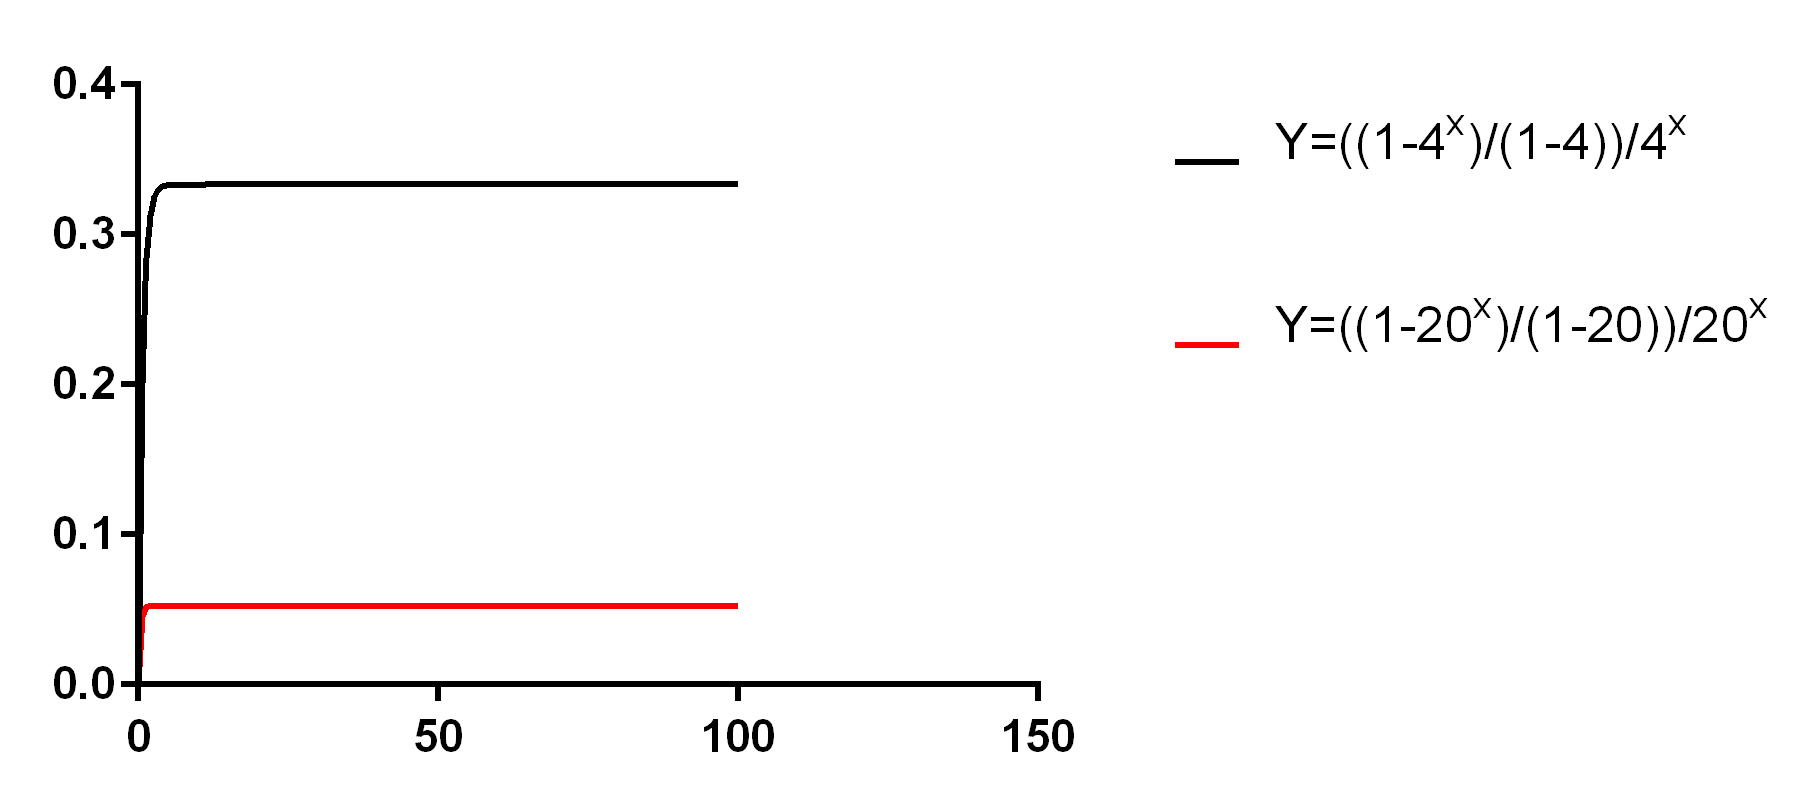
\includegraphics[scale=.60]{Graphs/Funciones1.png}
\caption{Razón entre sumatoria de progresión y último término}\label{graf1}
\end{figure}

Como observé que el valor de $x$ rápidamente llegaba a su asíntota decidí modificar la variable de independiente: 
\begin{figure}[H]
\centering
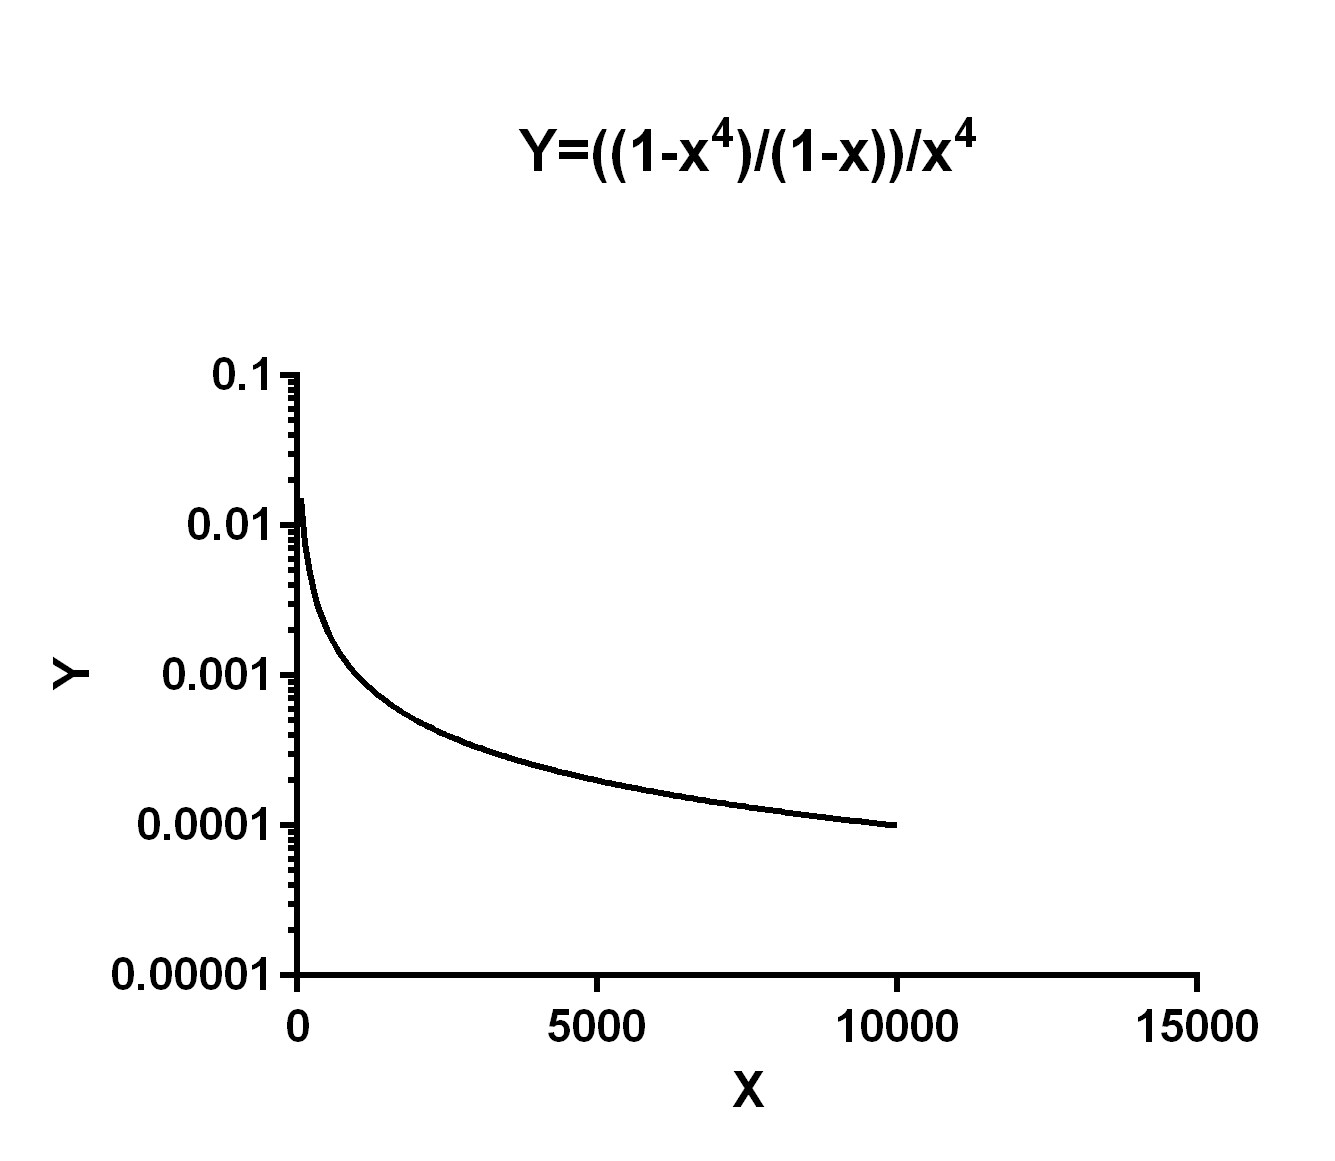
\includegraphics[scale=.60]{Graphs/Funciones2.png}
\caption{Razón entre sumatoria de progresión y último término}\label{graf1}
\end{figure}

De esta aproximación describí el comportamiento asintótico del algoritmo con la siguiente función:
\begin{equation}
f(x) = 4^{(9-x)}
\end{equation}
Ya que según los datos de mi programa, $4$ fue el promedio de ramificaciones del árbol de juego y 9 es el número máximo de turnos, que representa la \emph{profundidad} del árbol. Para obtener una mejor correlación con la gráfica, posteriormente ajusté este valor\footnote{Lo que se justifica al considerar que el número de subárboles de una sola rama es exponencialmente mayor al resto, según nuestra anterior función}, y obtuve un mejor aproximado del valor de ramificación de $4.5511$: 
\begin{figure}[H]
\centering
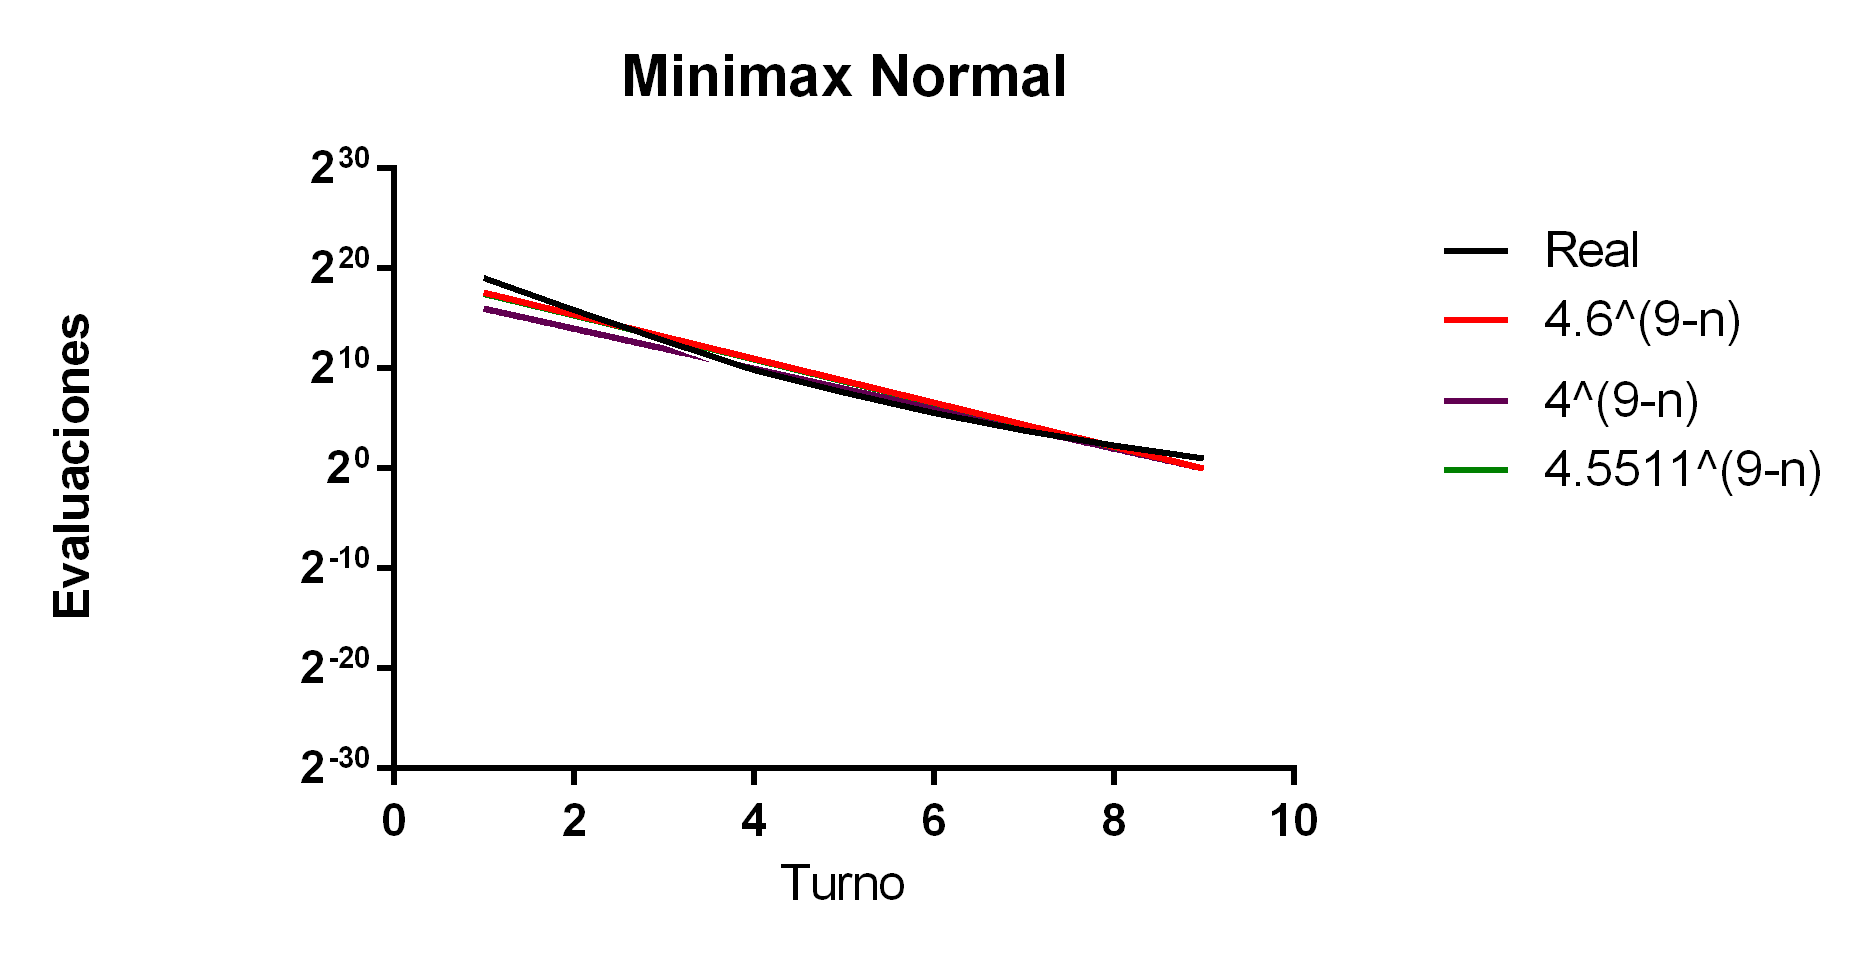
\includegraphics[scale=.60]{Graphs/Minis_Exposimples.png}
\caption{Comportamiento asíntotico de Minimax}\label{graf2}
\end{figure}

Posteriormente, realicé el mismo procedimiento con la optimizacíón alfa-beta\ref{alg:alfaBeta}, partiendo de la premisa de que ofrece ĺa siguiente complejidad asintótica en el mejor escenario $O(b^{(d/2))}$\autocite{bruce_cs_} y ajustando el valor multiplicativo para alcanzar un mejor ajuste: 
\begin{figure}[H]
\centering
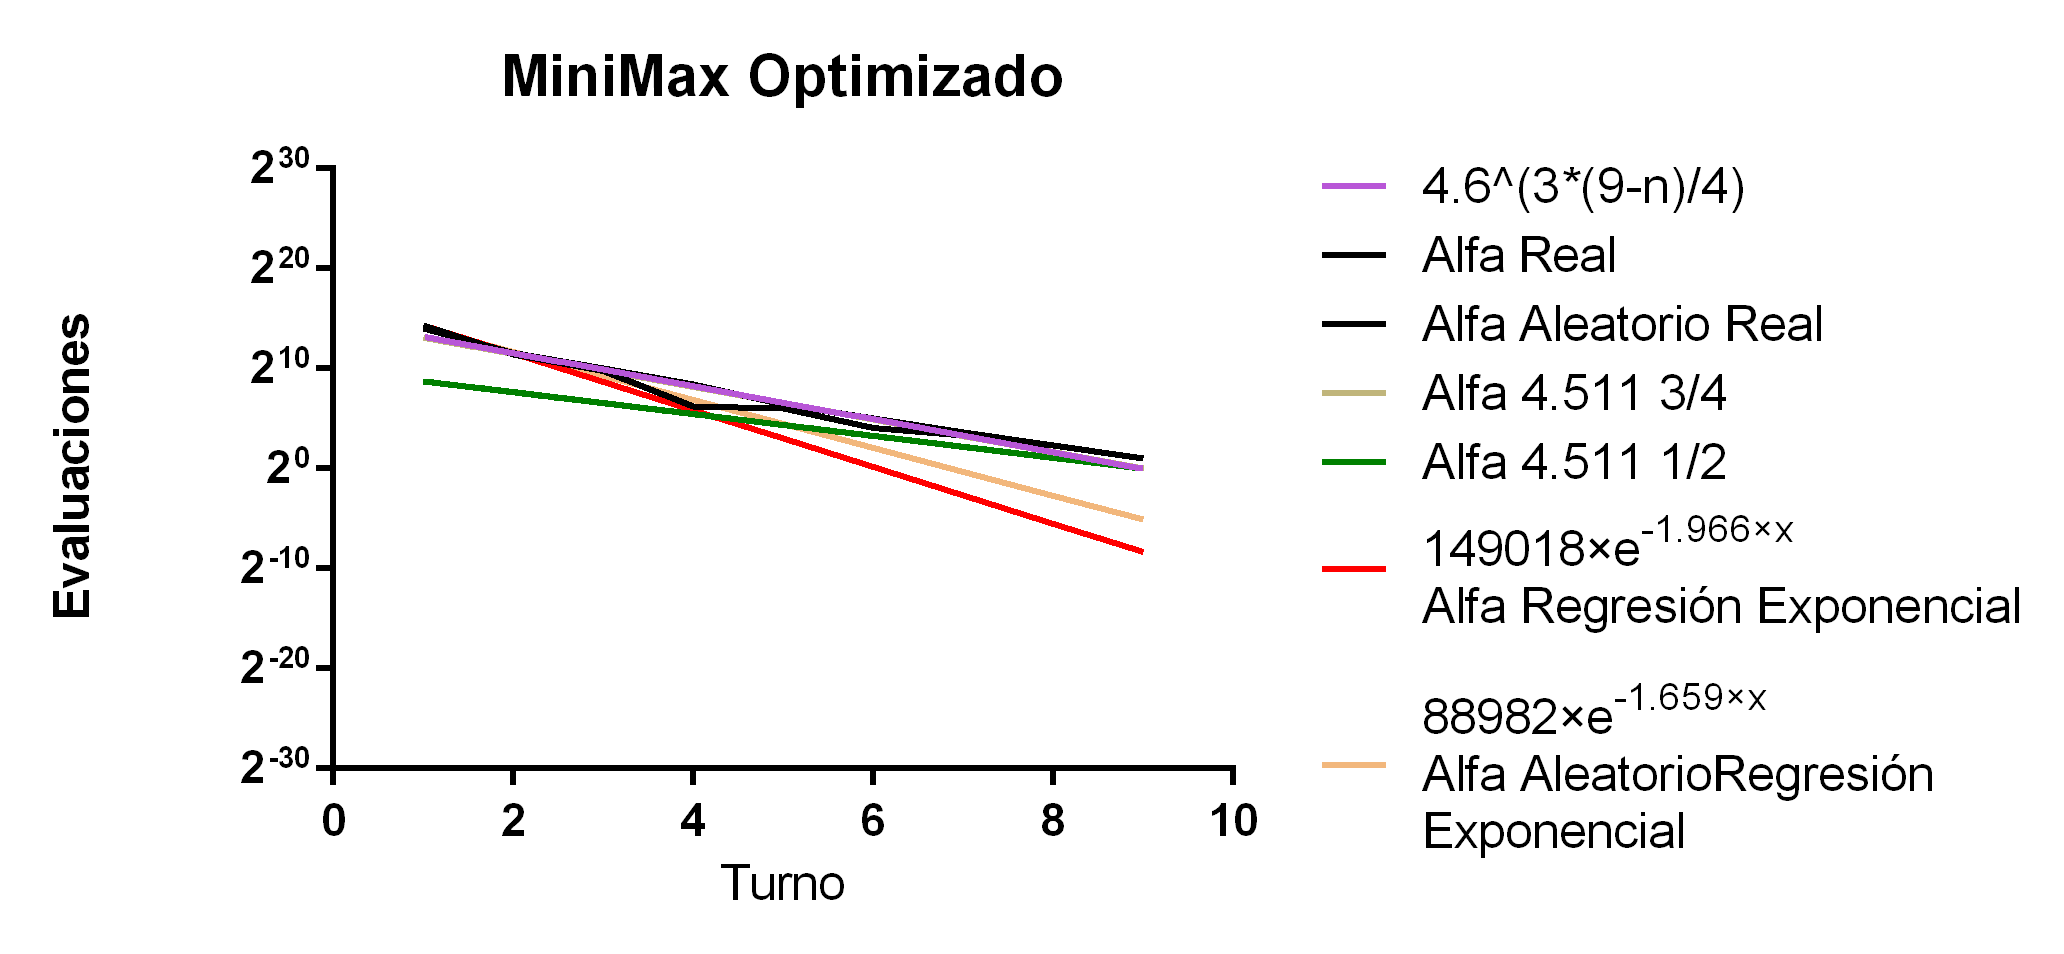
\includegraphics[scale=.60]{Graphs/Alfas.png}
\caption{Comportamiento asíntotico de AlfaBeta}\label{graf2}
\end{figure}

La función que grafiqué previo a realizar un ajuste con el método de menor número de cuadrados fue  la siguiente:

\begin{equation}
f(x) = 4^{(3*(9-x)/4)}
\end{equation}

\Section{Conclusión}
Debido a que MiniMax tiene un crecimiento exponencial, a pesar de su potencial para ofrecer estrategias óptimas, resulta inefectivo para juegos más complicados, ya que naturalmente tendrán una mayor profundidad y factor de ramificación. Por lo tanto, construir el árbol de juego tomaría una cantidad infactible de tiempo. Por lo tanto, la optimización alfa-beta resulta elemental para toda implementación de Minimax. Adicionalmente, podrían combinarse técnicas adicionales, para aproximar el valor real de alfa-beta hacia su óptimo de $O(b^{(d/2)})$, además, miniMax\ref{alg:MiniMax} puede ser modificado para evaluar de manera heurística el juego sin completar la construcción del árbol.